\begin{wrapfigure}[8]{l}{7cm}
  \centering
  \vspace{-4mm}
  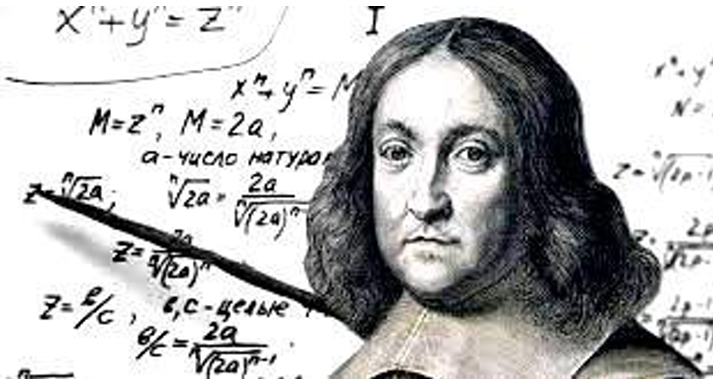
\includegraphics[width=0.4\textwidth]{Figures/P3/Fig 3.1.png}
\end{wrapfigure}

\noindent Nguyên lý Fermat là cơ sở quan trọng của quang hình học, theo đó, đường truyền ánh sáng luôn là đường truyền sao cho thời gian truyền sáng là ngắn nhất. Nguyên lý này được Heron thành Alexandria phát biểu lần đầu vào thế kỷ I để giải thích hiện tượng phản xạ ánh sáng và được Pierre Fermat phát biểu vào năm 1662 dưới dạng một định luật tổng quát nhất của quang hình học.\\
\indent Nguyên lý Fermat từng được coi là một bí ẩn của khoa học: "Tại sao ánh sáng có thể tìm được đường đi nhanh nhất? Liệu ánh sáng có một bộ não nào đó?". Tất nhiên, ánh sáng không có não, nhưng hãy chứng minh rằng, bạn thì có!\\
\indent Trong bài này, bạn cần giải quyết một số bài toán quang học bằng cách sử dụng nguyên lý Fermat. Giả sử rằng bạn không biết các định luật về phản xạ và khúc xạ ánh sáng, nhưng bạn biết và tin vào nguyên lý Fermat. Bạn vẫn được phép sử dụng định luật truyền thẳng của ánh sáng. Trong các bài toán liên quan đến gương và thấu kính, hãy sử dụng phép xấp xỉ paraxial, tức hãy xem như các tia sáng di chuyển lân cận quang trục và tạo với quang trục các góc nhỏ.
\subsection*{Phần 1: Giới thiệu Toán học}
\noindent Để đơn giản hoá các thao tác tính toán, hãy sử dụng các công thức toán học sau:
\begin{enumerate}
  \item Chứng minh rằng khi $x\ll a$, ta sẽ có:
        \begin{equation}
          \label{eq:p31}
          \sqrt{a^{2}+x^{2}}\approx a+\frac{x^{2}}{2a}
        \end{equation}
  \item Một cung tròn nhỏ có thể xem gần đúng như một đoạn parabol. Xét một đường tròn bán kính $R$ có tâm nằm trên trục $y$ và đường tròn tiếp xúc với trục $x$. Chỉ ra rằng, phương trình của parabol tiếp xúc với đường tròn tại gốc toạ độ có dạng:
        \begin{equation}
          \label{eq:p32}
          y=\frac{x^{2}}{2R}
        \end{equation}
\end{enumerate}
Ngay cả khi bạn không thể chứng minh các công thức \eqref{eq:p31} và \eqref{eq:p32}, bạn vẫn có thể sử dụng chúng trong các phần tiếp theo.

\begin{figure}[h]
  \centering
  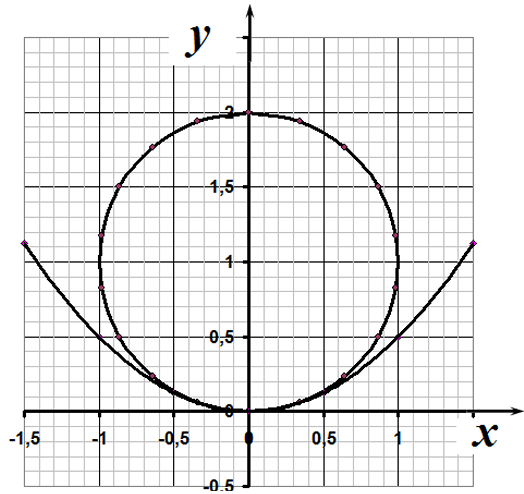
\includegraphics[width=0.3\textwidth]{Figures/P3/Fig 3.2.png}
\end{figure}

\subsection*{Phần 2: Sự đẳng thời}
\begin{wrapfigure}[8]{r}{8cm}
  \centering
  \vspace{-4mm}
  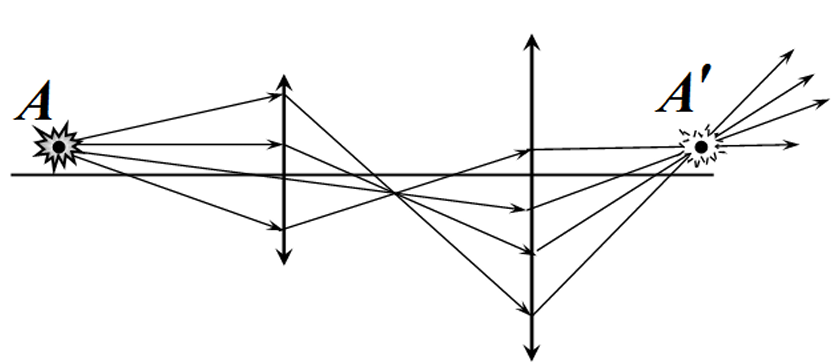
\includegraphics[width=0.45\textwidth]{Figures/P3/Fig 3.3.png}
\end{wrapfigure}

\noindent Một trường hợp cụ thể của nguyên lý Fermat là nguyên lý đẳng thời (hay nguyên lý Tautochronism). Nguyên lý này khẳng định rằng, với bất kì hệ quang học nào tạo ra ảnh, thời gian ánh sáng truyền từ nguồn điểm $A$ đến ảnh $A'$ của nó dọc theo bất kì con đường nào đều như nhau. Nói cánh khác, thời gian ánh sáng truyền từ nguồn $A$ đến ảnh $A'$ không phụ thuộc vào đường truyền ánh sáng.
\begin{enumerate}
  \item Cho một gương cầu lõm có bán kính $R$, tâm hình học $O$, quang tâm $C$ và quang trục $OC$ (Hình 3a). Bằng cách sử dụng nguyên lý đẳng thời, hãy chỉ ra rằng tất cả các tia $A'A$ song song với quang trục sau khi phản xạ trên gương sẽ giao nhau tại một điểm $F$ được gọi là tiêu điểm. Tìm tiêu cự $f=FC$ của gương.
  \item Cho một thấu kính phẳng lồi có bán kính cong của mặt lồi là $R$ và chiết suất của vật liệu làm thấu kính là $n$. $O$ là tâm hình học của mặt lồi và $C$ là quang tâm của thấu kính. $OC$ là quang trục của thấu kính (hình 3b). Bằng cách sử dụng nguyên lý đẳng thời, hãy chỉ ra rằng tất cả các tia $A'A$ song song với quang trục sau khi phản xạ trên gương sẽ giao nhau tại một điểm $F$ được gọi là tiêu điểm. Tìm tiêu cự $f=FC$ của thấu kính.
  \item Trên quang trục của một gương cầu lõm bán kính $R$ có đặt một nguồn sáng điểm $A$ ở khoảng cách $a=AC$ tính từ quang tâm của gương. Ảnh của điểm sáng này nằm ở khoảng cách $b=BC$ tính từ quang tâm của gương (hình 3c).
        \begin{enumerate}
          \item[a.] Sử dụng nguyên lý đẳng thời, chứng minh ảnh của điểm sáng này là ảnh thật.
          \item[b.] Thiết lập biểu thức biểu diễn mối quan hệ giữa $a,b$ và tiêu cự $f$ của gương. Biểu thức mà bạn tìm được gọi là "công thức gương cầu lõm"
        \end{enumerate}
  \item  Như bạn đã biết, các ảnh có thể là ảo (hình 3d).
        \begin{itemize}
          \item[a.] Cải tiến nguyên lý đẳng thời sao cho ta có thể dùng nó để xác định vị trí của các ảnh ảo.
          \item[b.] Chứng minh "công thức gương cầu lồi" có thể được viết dưới dạng tương tự "công thức gương cầu lõm" nếu bạn định nghĩa lại các đại lượng trong công thức đó.
          \item[c.] Giải thích nguyên lý đẳng thời bằng các lập luận trong phạm vi không quá 100 từ.
        \end{itemize}
\end{enumerate}


\begin{figure*}
  \centering
  \begin{subfigure}[b]{0.475\textwidth}
    \centering
    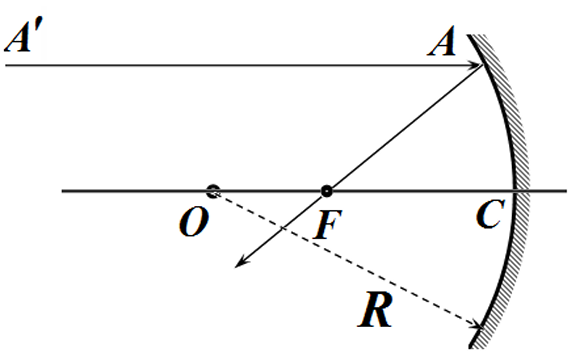
\includegraphics[width=0.7\textwidth]{Figures/P3/Fig 3.4.png}
    \caption{}
  \end{subfigure}
  \hfill
  \begin{subfigure}[b]{0.475\textwidth}
    \centering
    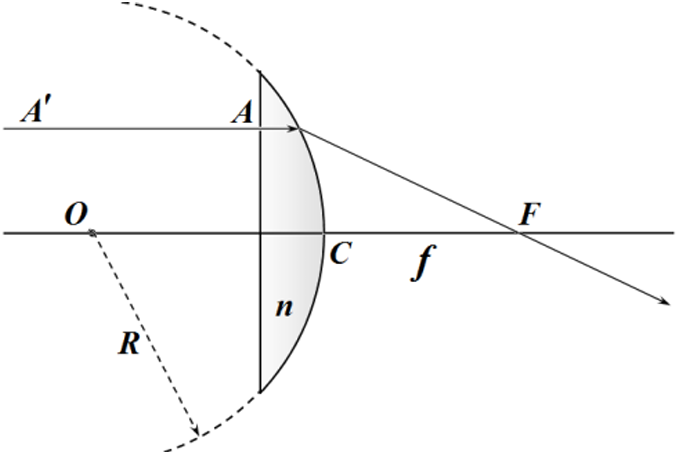
\includegraphics[width=0.85\textwidth]{Figures/P3/Fig 3.5.png}
    \caption{}
  \end{subfigure}
  \vskip\baselineskip
  \begin{subfigure}[b]{0.475\textwidth}
    \centering
    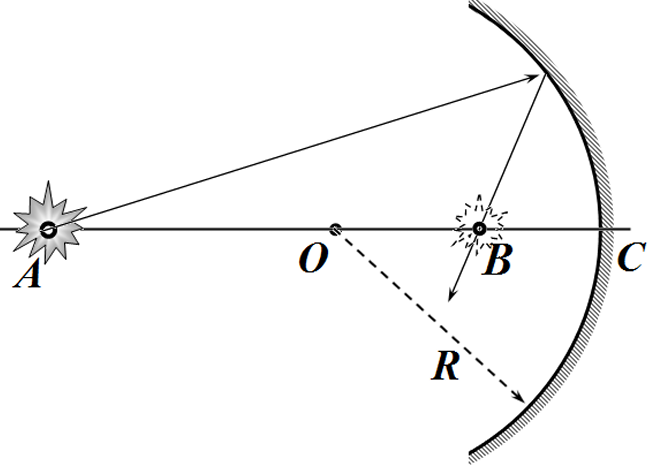
\includegraphics[width=0.8\textwidth]{Figures/P3/Fig 3.6.png}
    \caption{}
  \end{subfigure}
  \hfill
  \begin{subfigure}[b]{0.475\textwidth}
    \centering
    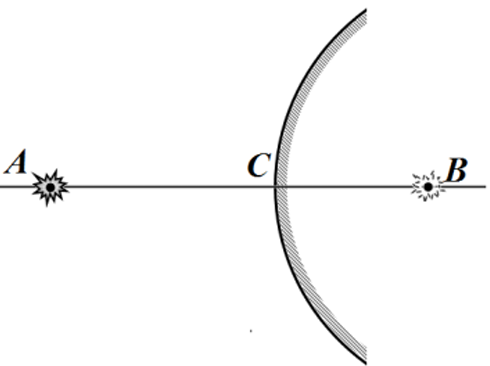
\includegraphics[width=0.8\textwidth]{Figures/P3/Fig 3.7.png}
    \caption{}
  \end{subfigure}
  \begin{center}
    \figurename{ 3}
  \end{center}
\end{figure*}

\subsection*{Phần 3: Nguyên lý Fermat}
\begin{enumerate}
  \item Điểm $A$ nằm trong môi trường có chiết suất $n_{1}$, điểm $B$ nằm trong môi trường có chiết suất $n_{2}$. Một tia sáng xuất phát từ $A$, sau khi khúc xạ qua mặt phân cách, sẽ đi đến $B$. Sử dụng nguyên lý Fermat, thiết lập công thức cho định luật khúc xạ ánh sáng.
  \item Cho một ống trụ rỗng có bán kính $R$, mặt trong của lớp trụ được mạ bạc nhờ đó ánh sáng có thể phản xạ trên nó. Khảo sát sự phản xạ của một tia sáng bên trong ống trụ trong mặt phẳng vuông góc với trục đối xứng của ống, chỉ ra tất cả các quỹ đạo khả dĩ của tia sáng $ACB$. Các điểm $A, B, C$ đều nằm trên mặt trong của ống trụ. Tâm của mặt cắt là $O$ và vị trí của điểm $C$ được xác định bởi góc $\phi$.
        \begin{enumerate}
          \item[a.] Xác định biểu thức của chiều dài quỹ đạo $ACB$ theo góc $\phi$ - $L(\phi)$. Phác hoạ đồ thị biểu diễn sự phụ thuộc này cho tất cả các giá trị khả thi của $\phi$.
          \item[b.] Xác định các giá trị của góc $\phi$ ứng với quỹ đạo thực của tia sáng. Chỉ ra các giá trị này trên đồ thị $L-\phi$.
        \end{enumerate}
\end{enumerate}

\begin{figure}[h]
  \centering
  \begin{subfigure}[b]{0.49\textwidth}
    \centering
    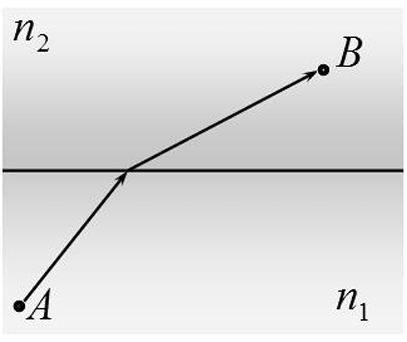
\includegraphics[width=0.7\textwidth]{Figures/P3/Fig 3.8.png}
  \end{subfigure}
  \hfill
  \begin{subfigure}[b]{0.49\textwidth}
    \centering
    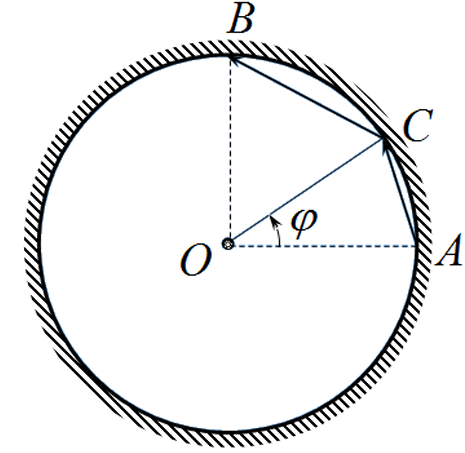
\includegraphics[width=0.7\textwidth]{Figures/P3/Fig 3.9.png}
  \end{subfigure}
\end{figure}

\begin{enumerate}
  \setcounter{enumi}{2}
  \item Các kết luận:
        \begin{enumerate}
          \item[a.] Cải tiến công thức của nguyên lý Fermat để có thể mô tả tất cả các trường hợp đã khảo sát trong bài này.
          \item[b.] Lí giải bằng lời nguyên lý Fermat trong phạm vi không quá 100 từ.
        \end{enumerate}
\end{enumerate}